\documentclass[conference]{IEEEtran}
\IEEEoverridecommandlockouts
% The preceding line is only needed to identify funding in the first footnote. If that is unneeded, please comment it out.
\makeatletter
\def\endthebibliography{%
	\def\@noitemerr{\@latex@warning{Empty `thebibliography' environment}}%
	\endlist
}
\makeatother
\usepackage{cite}
\usepackage{amsmath,amssymb,amsfonts}
\usepackage{algorithmic}
\usepackage{hyperref}
\usepackage{graphicx}
\usepackage{textcomp}
\usepackage{xcolor}
\usepackage{adjustbox}
\usepackage{multirow}
\usepackage{subcaption}
\def\BibTeX{{\rm B\kern-.05em{\sc i\kern-.025em b}\kern-.08em
		T\kern-.1667em\lower.7ex\hbox{E}\kern-.125emX}}
\begin{document}
	
	\title{Deteksi Pejalan Kaki pada \textit{Zebracross} untuk Peringatan Dini Pejalan Kaki menggunakan Mask R-CNN}
	
	\makeatletter
	\newcommand{\linebreakand}{%
	\end{@IEEEauthorhalign}
	\hfill\mbox{}\par
	\mbox{}\hfill\begin{@IEEEauthorhalign}
	}
	\makeatother
	
	\author{
		\centering
		
		\IEEEauthorblockN{1\textsuperscript{st}Mauridhi Hery Purnomo}
		\IEEEauthorblockA{\textit{Department of Computer Engineering} \\
			\textit{Faculty of Intelligent Electrical}\\
			\textit{and Informatics Technology}\\
			\textit{Institut Teknologi Sepuluh Nopember}\\
			Surabaya, Indonesia 60111 \\
			hery@ee.its.ac.id}
		\and
		\IEEEauthorblockN{2\textsuperscript{nd}Eko Mulyanto Yuniarno}
		\IEEEauthorblockA{\textit{Department of Computer Engineering} \\
			\textit{Faculty of Intelligent Electrical}\\
			\textit{and Informatics Technology}\\
			\textit{Institut Teknologi Sepuluh Nopember}\\
			Surabaya, Indonesia 60111 \\
			ekomulyanto@ee.its.ac.id}
		\and
		\IEEEauthorblockN{3\textsuperscript{rd} Agung Wicaksono}
		\IEEEauthorblockA{\textit{Department of Computer Engineering} \\
			\textit{Faculty of Intelligent Electrical}\\
			\textit{and Informatics Technology}\\
			\textit{Institut Teknologi Sepuluh Nopember}\\
			Surabaya, Indonesia 60111 \\
			agung.17072@mhs.its.ac.id}
		
	}
	
	\maketitle
	
	
	\begin{abstract}
		\textit{Dewasa ini, fitur keselamatan pada kendaraan roda empat atau mobil sudah sangat berkembang pesat. Hal tersebut terbukti dengan banyaknya produsen mobil yang menerapkan teknologi seat belt, air bag, adaptive cruise control, electronic stability control, autonomous emergency braking, blind spot monitoring dan lain sebagainya. Namun, fitur yang sudah disebutkan diatas dinilai masih kurang ramah bagi pejalan kaki. Terbukti menurut data dari WHO, terdapat 270.000 pejalan kaki meninggal dunia setiap tahun atau sekitar 22\% dari seluruh korban meniggal akibat kecelakan di jalan. Berawal dari permasalahan tersebut, penulis akan melakukan penelitian mengenai pendeteksian pejalan kaki pada zebracross untuk peringatan dini pengendara mobil sebagai topik penelitian. Pada tugas akhir ini, terdapat 3 objek yang akan dideteksi yaitu pejalan kaki, zebracross dan pengendara motor dengan menggunakan metode Mask R-CNN. Hasil terbaik yang didapatkan adalah pada penggunaan \textit{ResNet-101} untuk \textit{backbone Mask R-CNN} dengan skor \textit{mAP} sebesar 76.605\%, mAR sebesar 85.375\% serta \textit{F1-Score} sebesar 80.302\% .}
	\end{abstract}
	\begin{IEEEkeywords}
		\textit{Pejalan Kaki, Zebracross, Mask R-CNN, Pengolahan Citra}
	\end{IEEEkeywords}
	
	\section{Latar Belakang}
	\IEEEPARstart{M}{obil} merupakan salah satu jenis kendaraan bermotor yang banyak terdapat di Indonesia. Pada tahun 2018 Badan Pusat Statistik mencatat terdapat 16.440.987 mobil penumpang yang berada di In donesia. Dengan bertambahnya jumlah mobil di Indonesia dari tahun ke tahun, meningkatkan juga jumlah kecelakaan mobil. Fitur keselamatan dan keamanan pada mobil sangat penting bagi para pen gendara dan penumpang, sehingga para produsen mobil berusaha meningkatkan teknologi keselamatan dan keamanan pada mobil buatannya. Sebagai contoh beberapa fitur keselamatan dan keamanan yang terdapat pada mobil antara lain, adaptive cruise control, hill strat assist, blind spot monitoring, electronic stability control dan lain sebagainya.\cite{cit:1}
	
	
	\vspace{1ex}
	
	Menurut data dari WHO, terdapat 270.000 pejalan kaki meninggal dunia setiap tahun atau sekitar 22\% dari seluruh korban meniggal akibat kecelakan di jalan. Melihat kegiatan para pejalan kaki yang jarang berada di badan jalan, angka tersebut tentu cukup tinggi. Para pejalan kaki hanya menggunakan badan jalan ketika hendak menyebrang jalan lewat zebracross. Kelalaian dari pejalan kaki maupun pengendara mobil merupakan faktor utama mengapa angka kematian pejalan kaki cukup tinggi. Salah satu contoh kelalaian pejalan kaki adalah pada saat menyebrang jalan tidak memperhatikan kendaraan yang akan lewat dan atau melihat rambu serta lampu lalu lintas. Di sisi pengendara mobil, kelelahan, kurangnya fokus saat berkendara dan tidak memperhatikan rambu maupun marka dapat berakibat fatal baik kepada pejalan kaki dan pengendara lain. \cite{cit:4}.
	
	\vspace{1ex}
	
	Teknologi artificial intelligent sudah banyak disematkan pada mobil pada masa kini, dibuktikan dengan adanya teknologi adaptive cruise control, hill start assist dan lain sebagainya. Artificial intelligent khususnya deep learning tentu dapat digunakan untuk deteksi pejalan kaki di zebracross guna mengurangi jumlah korban akibat kecelakaan. Deteksi pejalan kaki dapat digabungkan dengan buzzer dan atau LED sebagai komponen output untuk mengingatkan kepada pengendara bahwa ada pejalan kaki yang sedang menyebrangi jalan serta mengembalikan fokus untuk berkendara.
	
	\vspace{1ex} 
	
	Penelitian mengenai deteksi pejalan kaki di jalan raya sudah ada sebelumnya seperti Real-Time Pedes trian Detection With Deep Network Cascades (Anelia Angelova et al.) \cite{cit:1}, dimana pada penelitian ini dihasilkan average miss rate sebesar 26,2\% yang berjalan secara real time. Selanjutnya terdapat peneli tian yang berjudul Pedestrian Detection: The Elephant In The Room (Irtiza Hasan et al.). \cite{cit:2}. Pada penelitian ini membandingkan antara detektor objek secara umum yaitu Cascade R-CNN dengan detek tor objek khusus pejalan kaki pada dataset yang berbeda. Pada penelitian yang berjudul Fast Vehicle and Pedestrian Detection Using Improved Mask R-CNN Vincent Vanhoucke (Chenchen Xu et al.). \cite{cit:3} dijelaskan mengenai deteksi terhadap kendaraan yang bergerak dan pejalan kaki. Penggunaan Restnet 86 untuk menggantikan Restnet-101 sebagai backbone membuat deteksi lebih akurat pada dataset yang terdapat pada MS COCO. Pada MASK R-CNN for Pedestrian Crosswalk Detection and Instance Segmen tation (Mon Arjay Malbog). \cite{cit:4} deteksi hanya dilakukan pada pedestrian crosswalk atau zebracross saja. Taining data dilakukan dengan Mask R-CNN untuk deteksi objek serta Restnet-101 sebagai backbone. Selanjutnya pada A Pedestrian Detection and Tracking System Based on Video Processing Technology (Chen, Yuanyuan et al.) \cite{cit:5}. dijelaskan mengenai deteksi pada pejalan kaki, pelacakan penghitungan serta peringatan resiko pada sebuah segemen video. 
	
	\section{Desain dan Implementasi Sistem}
	\vspace{1ex}
	Pada \textit{paper} ini dijelaskan mengenai penerapan metode \textit{Deep Learning} yang bertujuan untuk mendeteksi dan mensegmentasikan adanya pejalan kaki yang sedang melewati \textit{zebracross} maupun berada disekitarnya. Gambar \ref{fig:1} menampilkan blok diagram dari sistem kerja yang digunakan untuk mendeteksi pejalan kaki pada \textit{zebracross}. Pada penelitian ini, digunakan dataset dari Caltech Pedestrian Dataset.
	\vspace{1ex}
	\begin{figure}[!ht] \centering
		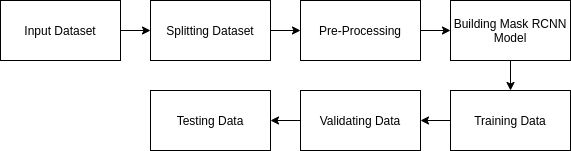
\includegraphics[width=0.4\textwidth]{img/blok-diagram.png}
		\caption{Blok Diagram Sistem Kerja}
		\label{fig:1}
	\end{figure}

	\subsection{Dataset yang Digunakan}
	\vspace{1ex}
	Pada penelitian ini, \textit{dataset} yang digunakan didapatkan dengan beberapa cara, antara lain:
	\begin{enumerate}
		\item \textit{Caltech Pedestrian Database}, merupakan kumpulan gambar yang diambil dari sudut pandang pengendara mobil di California Amerika Serikat dengan ukuran 640 x 480 pixel. Terdapat sekitar 250.000 gambar dengan 350.000 \textit{bounding boxes} dan sekitar 2.300 pejalan kaki dengan kriteria unik diberi tanda. Namun, pada \textit{dataset} ini hanya pejalan kaki saja yang diberi label, sehingga perlu dilakukan proses pelabelan ulang sesuai kelas yang diinginkan. Tidak semua gambar pada \textit{dataset} ini diambil untuk digunakan, gambar yang mempunyai objek berupa pejalan kaki dan \textit{zebracross} saja yang akan digunakan. Gambar \ref{fig:caltech} merupakan contoh dari gambar yang terdapat pada \textit{Caltech Pedestrian Database}.
		\begin{figure}[h]
			\centering
			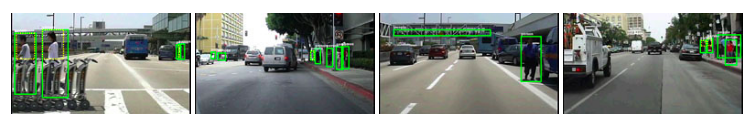
\includegraphics[scale=0.25]{img/caltech.png}
			\caption{Contoh Gambar dari Caltech Pedestrian Database}
			\label{fig:caltech}
		\end{figure} 
		
		\item Tangkapan layar dari beberapa video \textit{online Youtube}. Pada cara ini, penulis mencari video yang berada pada salah satu \textit{website video streaming} yaitu Youtube dengan persyaratan video diambil dari sudut pandang pengendara mobil yang berkendara pada jalan raya dengan ukuran gambar 1360x768 px. Pada \textit{frame-frame} tertentu dilakukan \textit{screenshot} dan disimpan untuk selanjutnya dilakukan proses pemberian label pada objek-objek yang diinginkan seperti pada Gambar \ref{fig:youtube-dataset}. 
		
		\begin{figure}[ht]
			\centering
			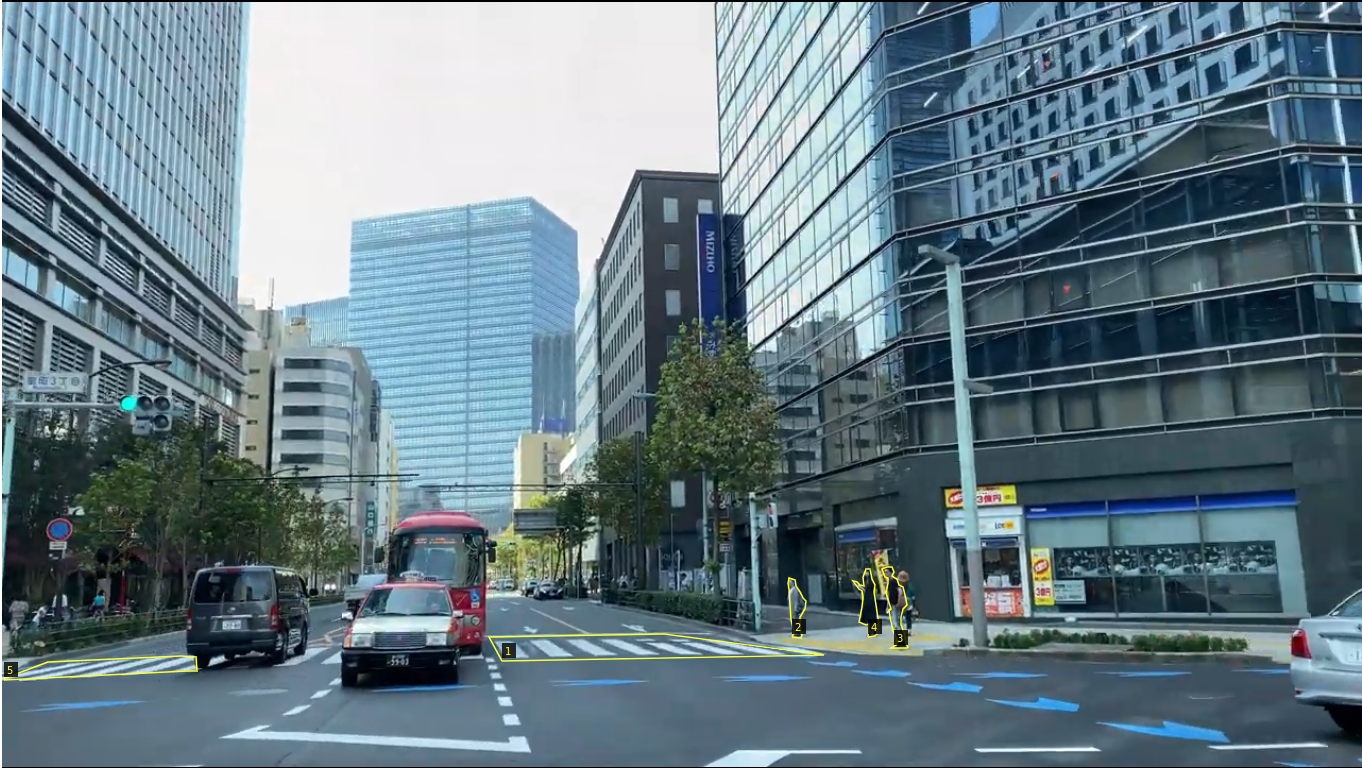
\includegraphics[scale=0.1]{img/youtube-dataset.png}
			\caption{Contoh Pembuatan \textit{dataset} dari \textit{Screenshot Youtube}}
			\label{fig:youtube-dataset}
		\end{figure}
		
		\item Pengambilan gambar secara mandiri menggunakan kamera \textit{smartphone} yang diambil dari sudut pandang pengendara motor dengan ukuran gambar yang diambil sebesar 1280x720 px. Pengambilan gambra dilakukan di jalan-jalan Surabaya. Setelah dilakukan pengambilan gambar, proses selanjutnya adalah pemberian label pada objek-objek yang ingin dideteksi.
	\end{enumerate}

	\vspace{1ex}
	Pada \textit{Machine Learning} dataset dibagi menjadi 3 bagian, yaitu dataset untuk keperluan \textit{training}, \textit{validation} dan \textit{testing}.
	\begin{enumerate}
		\item \textit{Training Set} digunakan pada proses \textit{learning} untuk melatih model dari algoritma yang sudah dibuat sebelumnya.
		\item \textit{Validatin Set} digunakan untuk mengukur kinerja dari model yang sudah dibuat dan menghindari terjadinya \textit{overfitting}
		\item \textit{Testing Set} digunakan untuk menguji keberhasilan dari model yang sudah dibuat.
	\end{enumerate}
	Pembagian rasio dataset pada \textit{paper} ini sebesar, 70\% untuk \textit{training}, 20\% untuk \textit{validation} dan 10\% untuk \textit{testing}.
	
	\subsection{Pemisahan Data}
	
	\vspace{1ex}
	Dalam \textit{machine learning} pemisahan data ke beberapa \textit{subset} merupakan suatu hal yang sangat penting. Hal ini dikarenakan setiap \textit{subset} memiliki fungsi masing-masing. Gambar \ref{fig:data-splitting} merupakan rasio pembagian data ke masing-masing subset.
	
	\begin{figure}[h]
		\centering
		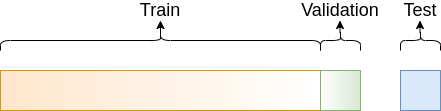
\includegraphics[scale=0.5]{img/data-splitting.png}
		\caption{Visualisasi Pembagian Data}
		\label{fig:data-splitting}
	\end{figure}
	
	\begin{enumerate}
		\item \textit{Training Sets}\\
		\textit{Training Sets} merupakan sampel data yang digunakan untuk melatih model yang sudah kita buat, dalam bidang \textit{Neural Network} bisa disebut juga bobot dan bias. Model yang sudah kita buat mempelajari pola masukan dan keluaran dari data ini. 
		
		\item \textit{Validation Sets}\\
		\textit{Validation Sets} merupakan sampel data yang digunakan untuk mengevaluasi model yang sudah dilatih menggunakan \textit{training sets}. Selain itu, data ini digunakan untuk memperbarui dan menyempurnakan hyperparameter dari model ke tingkat yang lebih tinggi.
		
		\item\textit{Test Sets}\\
		\textit{Test Sets} merupakan sampel data yang digunakan untuk mengevaluasi model akhir setelah melalui proses \textit{training dan validation}. Apabila pengujian model pada data ini sudah sesuai dengan yang diinginkan, maka proses \textit{learning} sudah selesai. Namun apabila pengujian tidak sesuai dengan yang diharapkan maka diperlukan pengaturan ulang mulai dari proses \textit{training}. 
	\end{enumerate} 
	
	\subsection{\textit{Pre-Processing}}
	\vspace{1ex}
	
	Pada tahap ini, gambar-gambar dari \textit{dataset} akan mengalami proses penyesuaian sebelum masuk ke proses \textit{data training}. Setiap gambar yang akan dijadikan bahan pembelajarnan model harus memiliki dimensi dan kedalaman yang sama. Tujuan dari \textit{pre processing} adalah perbaikan data gambar dengan menekan distorsi yang tidak diinginkan atau meningkatkan beberapa fitur gambar yang relevan untuk pemrosesan lebih lanjut. Gambar \ref{fig:preprocessing} merupakan tahapan dari \textit{pre-processing} gambar \textit{dataset} yang dilakukan.
	
	\begin{figure}[h]
		\centering
		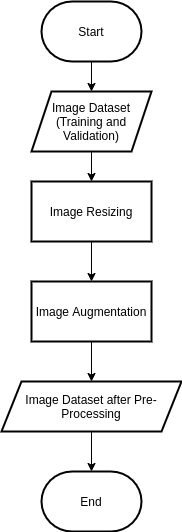
\includegraphics[scale=0.3]{img/flowchart-preprocessing.png}
		\caption{Diagram Alir \textit{Pre Processing}}
		\label{fig:preprocessing}
	\end{figure}
	
	Berikut merupakan penjelasan mengenai tahapan \textit{pre-processing} yang dilakukan pada penelitian kali ini:
	\begin{enumerate}
		\item \textit{Image resizing}\\
		Langkah awal dari proses \textit{pre-processing} adalah memastikan semua gambar dalam \textit{dataset} kita memiliki ukuran yang sama. Selain itu, sama seperti sebagian besar model dari \textit{neural network} lainnya, metode yang dilakukan penulis juga mengasumsikan gambar \textit{input} berbentuk persegi. Jadi diperlukan pemeriksaan gambar di awal, apakah gambar sudah berbentuk persegi atau belum. Berbeda dari metode \textit{image resizing} pada model \textit{neural network} lainnya yang menggunakan teknik \textit{cropping} untuk membuat aspek rasio gambar input menjadi persegi, penulis menggunakan metode yang sudah terdapat pada \textit{Mask R-CNN}.
		
		Ukuran gambar yang penulis pilih pada penelitian kali ini adalah 512x512 pixel. Pemilihan ukuran gambar ini dilakukan untuk mengurangi beban dan waktu saat \textit{training data}. Apabila terdapat gambar pada \textit{dataset} dengan ukuran baik panjang maupun lebar lebih dari 512 pixel. maka gambar akan di \textit{down scaling} sampai ukuran 512 pixel. Sebaliknya, apabila ada gambar pada \textit{dataset} dengan ukuran lebih kecil dari 512 pixel maka akan dilakukan \textit{up scaling} sampai gambar berukuran 512 pixel. Aspek rasio gambar yang sudah melalui proses \textit{scaling} tetap dipertahankan, namun diperlukan penambahan \textit{zero padding} untuk membuat gambar \textit{input} menjadi persegi seperti yang diinginkan.
		
		\begin{figure}[h]
			\centering
			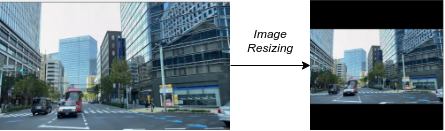
\includegraphics[scale=0.5]{img/image-resizing.png}
			\caption{Contoh \textit{Image Resizing}}
			\label{fig:image-resizing}
		\end{figure}
		
		Gambar \ref{fig:image-resizing} merupakan salah satu contoh \textit{image resizing} yang dilakukan. Gambar \textit{input} (gambar sebelah kiri) mempunyai ukuran 768x1360 dengan kedalaman 3 atau mempunyai format warna RGB. Setelah mengalami \textit{image resizing} (gambar sebelah kanan) ukuran gambar menjadi 290x512. Namun untuk membuat gambar memiliki aspek rasio 1:1 (berbetuk persegi) maka diperlukan penambahan \textit{zero padding} pada bagian atas gambar sebesar 111 pixel dan pada bagian bawah gambar sebesar 111 pixel. Dengan penambahn \textit{padding} seperti itu membuat gambar \textit{input} berbentuk persegi namun tidak mengurangi informasi gambar. 
		
		\item \textit{Image Augmentation}\\
		Langkah selanjutnya pada \textit{pre-processing} adalah \textit{image augmentaion}. Proses augmentasi yang dilakukan pada penelitian ini adalah rotasi dan transformasi. Tujuan dari penggunanaan \textit{image augmentation} adalah untuk mengekspos \textit{neural network} ke berbagai variasi, agar dapat mengenali fitur yang akan dilakukan pada proses \textit{training}. Hal tersebut akan sangat membantu \textit{neural network} untuk mengenali variasi yang tidak terdapat pada dataset. Seperti yang terdapat pada Gambar \ref{fig:image-augmentation}, tanpa ada augmentasi maka \textit{neural network} hanya mengenali satu kondisi saja. Jika memakai augmentasi gambar seperti transformasi, maka setidaknya \textit{neural network} akan dapat mengenali 2 kondisi. Semakin banyak augmentasi yang digunakan semakin banyak pula kondisi yang bisa dikenali oleh \textit{neural network}. Namun semakin banyak kondisi yang dikenali, semakin lama dan berat proses \textit{training data} yang dilakukan. 
		
		\begin{figure}[h]
			\centering
			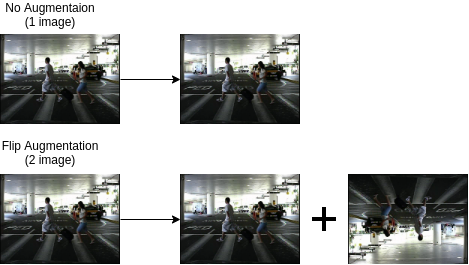
\includegraphics[scale=0.45]{img/image-augmentation.png}
			\caption{Contoh \textit{Image Augmentation}}
			\label{fig:image-augmentation}
		\end{figure}
		
	\end{enumerate}
	
	\subsection{Arsitektur Mask R-CNN}
	\vspace{1ex}
	Mask R-CNN merupakah salah satu metode \textit{deep lerning} yang dikembangkan dari Faster R-CNN dengan menambahkan satu cabang di tahap akhir untuk menghasilkan \textit{mask} dari objek yang dideteksi \cite{cit:11}. Pengembangan tersebut dilakukan untuk memecahkan masalah \textit{instance segmentation} yang terjadi dalam \textit{machine learning} dan pengolahan citra. Dengan kata lain, \textit{mask r-cnn}, dapat memisahkan objek yang berbeda walaupun dalam satu kelas yang sama pada gambar atau video. Selain memberikan hasil berupa \textit{bounding box} dan klasifikasi objek seperti kebanyakan algoritma \textit{object detection} lainnya, \textit{mask r-cnn} juga memberikan \textit{mask} dimana hal ini sangat bermanfaat pada segmentasi objek.
	
	\begin{figure}[ht]
		\centering
		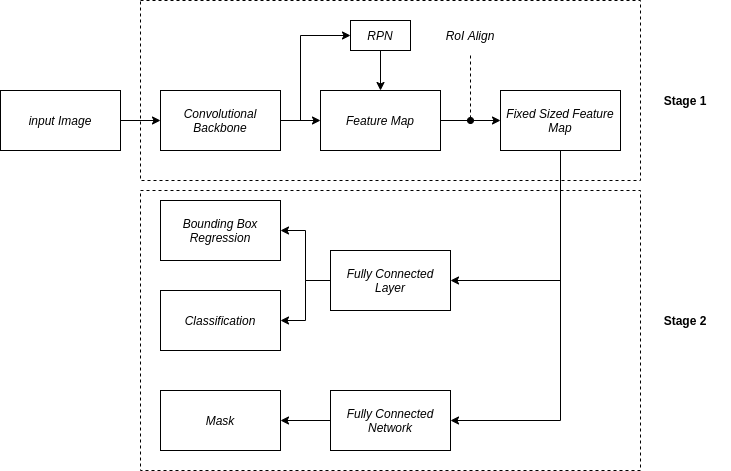
\includegraphics[scale=0.3]{img/mask-rcnn-arch.png}
		\caption{Blok Diagram Alur Mask R-CNN}
		\label{fig:mask-rcnn-arch}
	\end{figure} 
	
	Seperti yang ditampilkan pada Gambar \ref{fig:mask-rcnn-arch}, pada proses \textit{training} menggunakan \textit{mask r-cnn} dibagi menjadi 2 tahapan. Tahap pertama adalah tahap untuk menghasilkan proposal tentang area di mana mungkin ada objek berdasarkan gambar \textit{input}. Lalu tahap kedua adalah tahap untuk memprediksi kelas objek, memperbaiki \textit{bounding box} dan menghasilkan \textit{mask} di tingkat piksel objek berdasarkan proposal tahap pertama. Kedua tahap terhubung ke struktur \textit{backbone}.
	
	\textit{Backbone} adalah \textit{deep neural network} yang memiliki struktur seperti FPN (\textit{Feature Pyramid Network}). \textit{Backbone} terdiri dari \textit{bottom-up pathway}, \textit{up-bottom pathway} dan \textit{lateral connection}. \textit{Bottom-up pathway} dapat berupa berbagai jenis \textit{Convolutional Network}, biasanya berupa \textit{ResNet} atau \textit{VGG}, yang mengekstrak fitur dari \textit{raw images}. \textit{Up-bottom pathway} menghasilkan \textit{Feature Map Pyramid} yang ukurannya mirip dengan \textit{bottom-up pathway}. \textit{Lateral connection} adalah operasi konvolusi dan penjumlahan antara dua \textit{pathway} dengan tingkat yang sesuai. FPN mempunyai kinerja yang lebih baik dari ConvNet tunggal lainnya terutama karena FPN dapat mempertahankan fitur semantik yang sangat baik pada berbagai skala resolusi
	
	\subsection{Training Process}
	\vspace{1ex}
	Proses \textit{training data} dilakukan setelah pembuatan model telah selesai dan \textit{dataset} sudah melalui proses \textit{pre-processing}. Pada saat pertama kali menjalankan proses \textit{training}, bobot awal diambil dari \textit{pre-trained weight} yang sudah tersedia pada \textit{mask r-cnn}. Hal ini bisa dilakukan dengan menerapkan metode \textit{transfer learning}. \textit{Transfer learning} sendiri adalah teknik yang
	sangat efisien untuk melakukan proses \textit{training} atau \textit{retrain} pada \textit{neural network}. Penggunaan \textit{transfer learning} mempunyai keuntungan diantara lain proses \textit{training} pada data baru memakan waktu yang lebih cepat daripada memulai dari awal serta masalah dapat dipecahkan dengan menggunakan training data
	yang lebih sedikit daripada membangun model dari awal.
	
	Ada beberapa hal yang perlu diperhatikan dalam melakukan pengaturan saat akan menjalankan proses \textit{training} antara lain :
	\begin{enumerate}
		\item \textit{Iteration} adalah banyaknya proses yang dilakukan untuk melakukan \textit{forward} dan \textit{backward pass}. \textit{forward pass} adalah proses dimana \textit{output value} dari \textit{neural network} didapatkan setelah \textit{input value} dari \textit{input-neuron} telah selesai diproses. Sedangkan \textit{backward pass} adalah proses mengkalkulasikan bobot dari \textit{neural network} mulai dari \textit{output neuron} ke \textit{input neuron} untuk mendapatkan \textit{loss} dari setiap \textit{neuron}. Pada \textit{mask r-cnn iteration} bisa desebut juga dengan \textit{step\_per\_epoch} sesuai dengan yang tercantunm pada \textit{file} pengaturan \textit{mask r-cnn}. 
		
		\item \textit{Epoch}, ketika seluruh dataset sudah melalui proses \textit{training} pada \textit{neural network} sampai dikembalikan ke awal untuk sekali putaran. Sebagia contoh apabila kita menggunakan \textit{iteration} sebanyak 10 kali, maka satu \textit{epoch} sebanyak 10 \textit{iteration} dan kelipatannya. Pada penelitian kali ini penulis menggunakan \textit{epoch} sebanyak 100.
	\end{enumerate}

	\subsection{\textit{Validating Data}}
	\vspace{1ex}
	Setelah proses \textit{training} dilakukan, perlu dilakukan apakah model yang dibuat sudah memiliki tingkat akurasi sesuai yang kita inginkan dengang menggunakan teknik validasi.Pada proses inilah, \textit{dataset} yang telah dipisahkan pada proses sebelumnya akan berperan. Evaluasi memungkinkan pengujian model terhadap data yang belum pernah dilihat dan digunakan untuk pelatihan dan dimaksudkan untuk mewakili bagaimana model dapat menyelesaikan permasalahan tersebut. Tahapan pada validasi akan membantu untuk menemukan parameter terbaik untuk model prediktif dan mencegah dari \textit{overfitting}.
	
	Pada penelitian kali ini, digunakan salah satu jenis teknik validasi menggunakan \textit{Cross Validation}. Pada \textit{Cross Validation} data akan dibagi menjadi K lipatan, dimana setiap lipatan akan diambil satu data sebagai \textit{validation data} dan sisanya akan digunakan untuk \textit{training data}. Pemilihan \textit{validation data} dilakukan secara menyilang, dengan ketentuan apabila \textit{training} terjadi pada iterasi ke \textit{k} maka data yang dipilih untuk validasi adalah data \textit{k} juga. Gambar \ref{fig:cross-validation} merupakan visualisasi dari \textit{K Fold Cross Validation}.
	
	\begin{figure}[h]
		\centering
		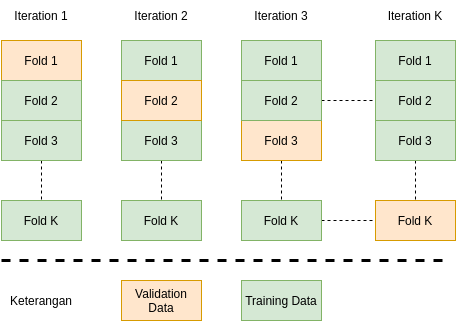
\includegraphics[scale=0.35]{img/cross-validation.png}
		\caption{Visualisasi \textit{K Fold Cross Validation}}
		\label{fig:cross-validation}
	\end{figure} 
	
	\subsection{Testing Process}
	\vspace{1ex}
	\textit{Testing data} merupakan tahap akhir dalam algoritma \textit{machine learning} secara umum. Pada tahap ini model akan diuji untuk didapatkan keakuratan untuk mendeteksi objek. Data uju yang digunakan pada tugas akhir kali ini adalah data yang berbentuk video. Jadi diperlukan \textit{pre-processing} yang berbeda dengan \textit{training data} dan \textit{validation data}. Data video akan dipecah atau dipotong-potong menjadi format gambar dengan ketentuan 30 \textit{frame per second}. Ketika \textit{data test} sudah dikonversi menjadi bentuk gambar, maka proses deteksi bisa dilakukan. Gambar hasil deteksi berupa gambar asli yang sudah ditambah dengan \textit{bounding box, classification, mask}. Lalu gambar-gambar tersebut disatukan lagi menjadi format video dengan ketentuan sama seperti saat pemotongan menjadi format gambar, yaitu 30 \textit{frame per second}. Gambar \ref{testing} merupakan diagram alir dari proses \textit{testing} dari model yang sudah dihasilkan dari proses \textit{training dan validation}.
	
	\begin{figure}[h]
		\centering
		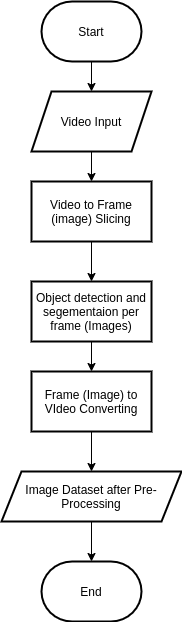
\includegraphics[scale=0.3]{img/testing.png}
		\caption{Diagram Alir Proses \textit{Testing}}
		\label{testing}
	\end{figure}
	
	
	\section{Testing and Result}
	
	\subsection{Hasil Training dan Validasi}
	\vspace{1ex}
	
	Setelah dilakukan serangkaian proses training didapatkan \textit{output} berupa \textit{model file}  dengan format \textit{h5}. \textit{Training loss} terendah yang berhasil dicapai dengan menggunakan \textit{backbone} Resnet-50 adalah 0.4061 dengan rincian \textit{training bounding box loss} sebesar 0.04083, \textit{training classification loss} sebesar 0.02268 serta \textit{training mask loss} sebesar 0.139 (dimana $L=L_{bbox}+L_{cls}+L_{mask}$). Sedangkan \textit{training loss} terendah yang berhasil dicapai dengan menggunakan \textit{backbone} Resnet-101 adalah 0.3933 dengan rincian \textit{training bounding box loss} sebesar 0.04164, \textit{training classification loss} sebesar 0.0247 serta \textit{training mask loss} sebesar 0.1403. Serta  \textit{training loss} terendah yang berhasil dicapai dengan menggunakan \textit{backbone} Mobilenet-V1 (pada \textit{epoch} ke 46) adalah 1.604 dengan rincian \textit{training bounding box loss} sebesar 0.2322, \textit{training classification loss} sebesar 0.07858 serta \textit{training mask loss} sebesar 0.6729. Gambar \ref{training-result} merupakan grafik yang menunjukkan perubahan \textit{training loss, training bounding box loss, training classification loss,} serta \textit{training mask loss} dari \textit{epoch} 1 sampai 300.
	
	\begin{figure}[h]
		\centering
		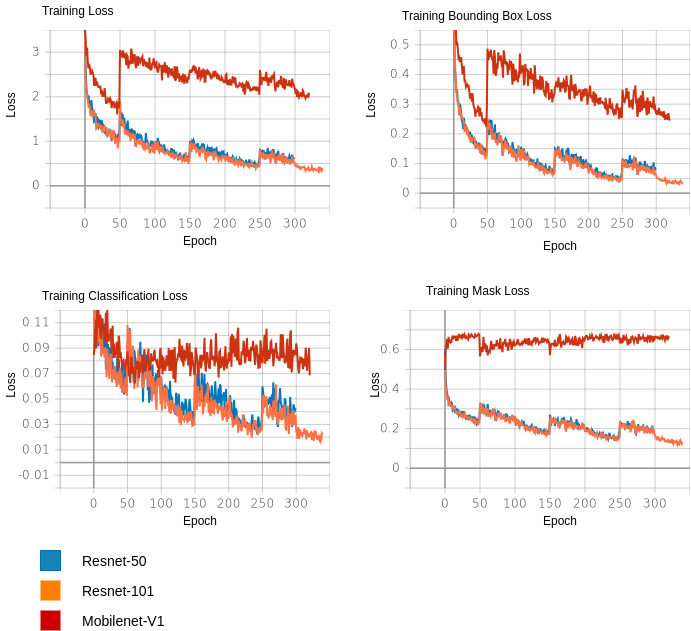
\includegraphics[scale=0.3]{img/training.png}
		\caption{Grafil Perubahan \textit{Training Loss}}
		\label{training-result}
	\end{figure} 

	Sedangkan pada saat proses \textit{validation} sendiri \textit{Loss} terendah yang berhasil dicapai menggunakan Resnet-50 adalah 0.3653 dengan rincian \textit{validation bounding box loss} sebesar 0.4556, \textit{validation classification loss} sebesar 0.01912 serta \textit{validation mask loss} sebesar 0.1519. Sedangkan \textit{validation} sendiri \textit{Loss} terendah yang berhasil dicapai menggunakan Resnet-101 adalah 0.299 dengan rincian \textit{validation bounding box loss} sebesar 0.03867, \textit{validation classification loss} sebesar 0.01246 serta \textit{validation mask loss} sebesar 0.1461. Serta \textit{validation} sendiri \textit{Loss} terendah yang berhasil dicapai menggunakan Mobilenet-V1 adalah 1.624 dengan rincian \textit{validation bounding box loss} sebesar 0.2088, \textit{validation classification loss} sebesar 0.04799 serta \textit{validation mask loss} sebesar 0.6001. Gambar \ref{validation} merupakan grafik yang menunjukkan perubahan \textit{validation loss, validation bounding box loss, validation classification loss,} serta \textit{validation mask loss} dari \textit{epoch} 1 sampai 300.
	
	\begin{figure}[h]
		\centering
		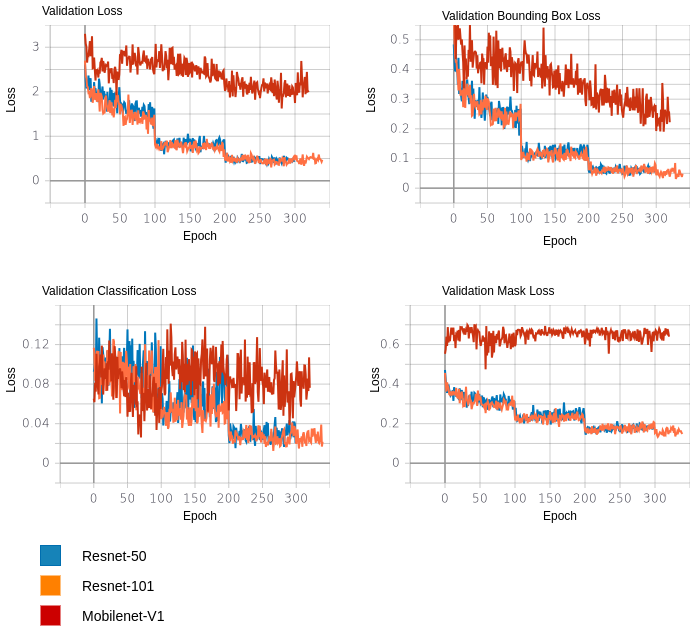
\includegraphics[scale=0.3]{img/validation.png}
		\caption{Grafil Perubahan \textit{Validation Loss}}
		\label{validation-result}
	\end{figure} 

	Selain menggunakan \textit{Loss Function} untuk mengukur peforma hasil \textit{training} yang sudah dilakukan, digunakan juga \textit{mean Average Precision (mAP)}. \textit{Precision} sendiri merupakan fungsi untuk menggambarkan tingkat keakuratan antara data yang diminta dengan hasil prediksi yang diberikan oleh model. Maka, \textit{precision} merupakan rasio prediksi benar positif (TP) dibandingkan dengan keseluruhan hasil yang diprediksi positif (TP dan FP). Rumus untuk mencari \textit{Precision} adalah sebagai berikut :
	\begin{equation}
		Precision = \frac{TP}{TP+FP} 
	\end{equation}
	
	Perhitungan \textit{mAP} pada penelitian ini dilakukan setiap 5 \textit{epoch} sekali, karena jika dilakukan setiap \textit{epoch} akan memerlukan \textit{training time} yang lebih lama serta \textit{resource hardware} yang diperlukan lebih besar. Nilai \textit{mAP} tertinggi didapatkan pada dengan menggunakan Resnet-50 adalah sebesar 94.92. Sedangkat pada Resnet-101 \textit{mAP} tertinggi yang berhasil dicapai sebesar 96.21 dan pada Mobilenet-V1 sebesar 26.04. Gambar \ref{map-result} merupakan grafik yang menunjukan perubahan \textit{validation mean Average Precision} dari \textit{epoch} 1 sampai 300.
	
	\begin{figure}[h]
		\centering
		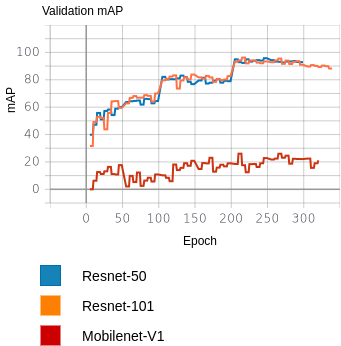
\includegraphics[scale=0.4]{img/map-result.png}
		\caption{Grafil Perubahan \textit{Validation Mean Average Precision}}
		\label{map-result}
	\end{figure}

	Tabel \ref{tab:training-result} adalah tabel perbandingan dari \textit{output file size}, \textit{mAP}, \textit{training time} dari total 3 model dengan \textit{backbone} berbeda yang diuji. 
	
	\begin{table}[h]
		\begin{tabular}{|c|l|c|c|l|}
			\hline
			\textbf{No} & \multicolumn{1}{c|}{\textit{\textbf{Backbone}}} & \textit{\textbf{Output File Size}} & \textit{\textbf{mAP}} & \multicolumn{1}{c|}{\textit{\textbf{Training Time}}} \\ \hline
			1           & Resnet-50                                       & 170.9 MB                                   & 94.92\%                      & 03:40:24                              \\ \hline
			2           & Resnet-101                                      & 244 MB                                    & 96.21\%                      & 04:09:16                                \\ \hline
			3           & Mobilenet-V1                                    & 83.3 MB                                    & 26.04\%                      & 03:18:44                              \\ \hline
		\end{tabular}
		\caption{Tabel Perbandingan Hasil \textit{Training}}
		\label{tab:training-result}
	\end{table}
	
	\subsection{Hasil Testing}
	\vspace{1ex}
	Proses \textit{testing} dilakukan menggunakan data dengan format gambar dan video dalam tiga kondisi yaitu pagi, siang dan malam hari. Pada \textit{testing} dengan menggunakan \textit{input} berupa gambar seperti yang tertampil pada Gambar \ref{fig:compare} didapatkan hasil seperti pada Tabel \ref{tab:result}
	\vspace{1ex}
	\begin{figure}[h]
		\centering
		\begin{minipage}[b]{0.2\textwidth}
			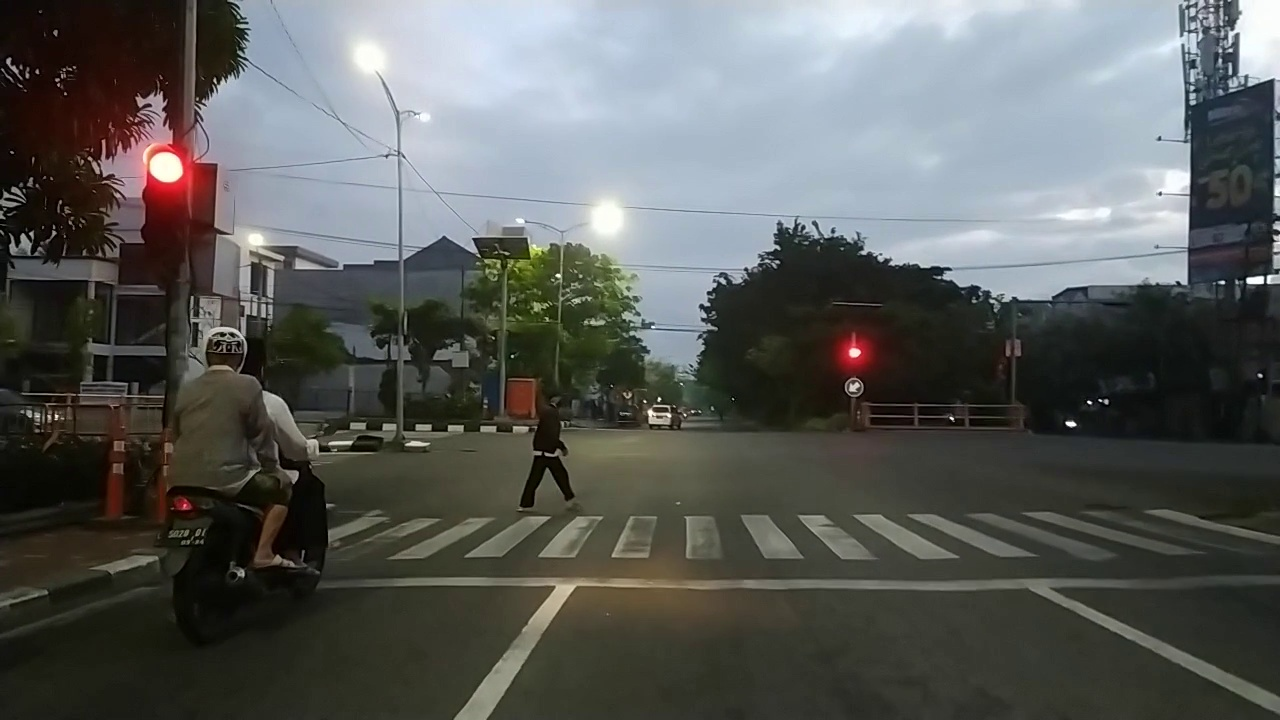
\includegraphics[width=\textwidth]{img/frame800.jpg}
			\caption*{(a) Pagi}
		\end{minipage}
		\hfill
		\begin{minipage}[b]{0.2\textwidth}
			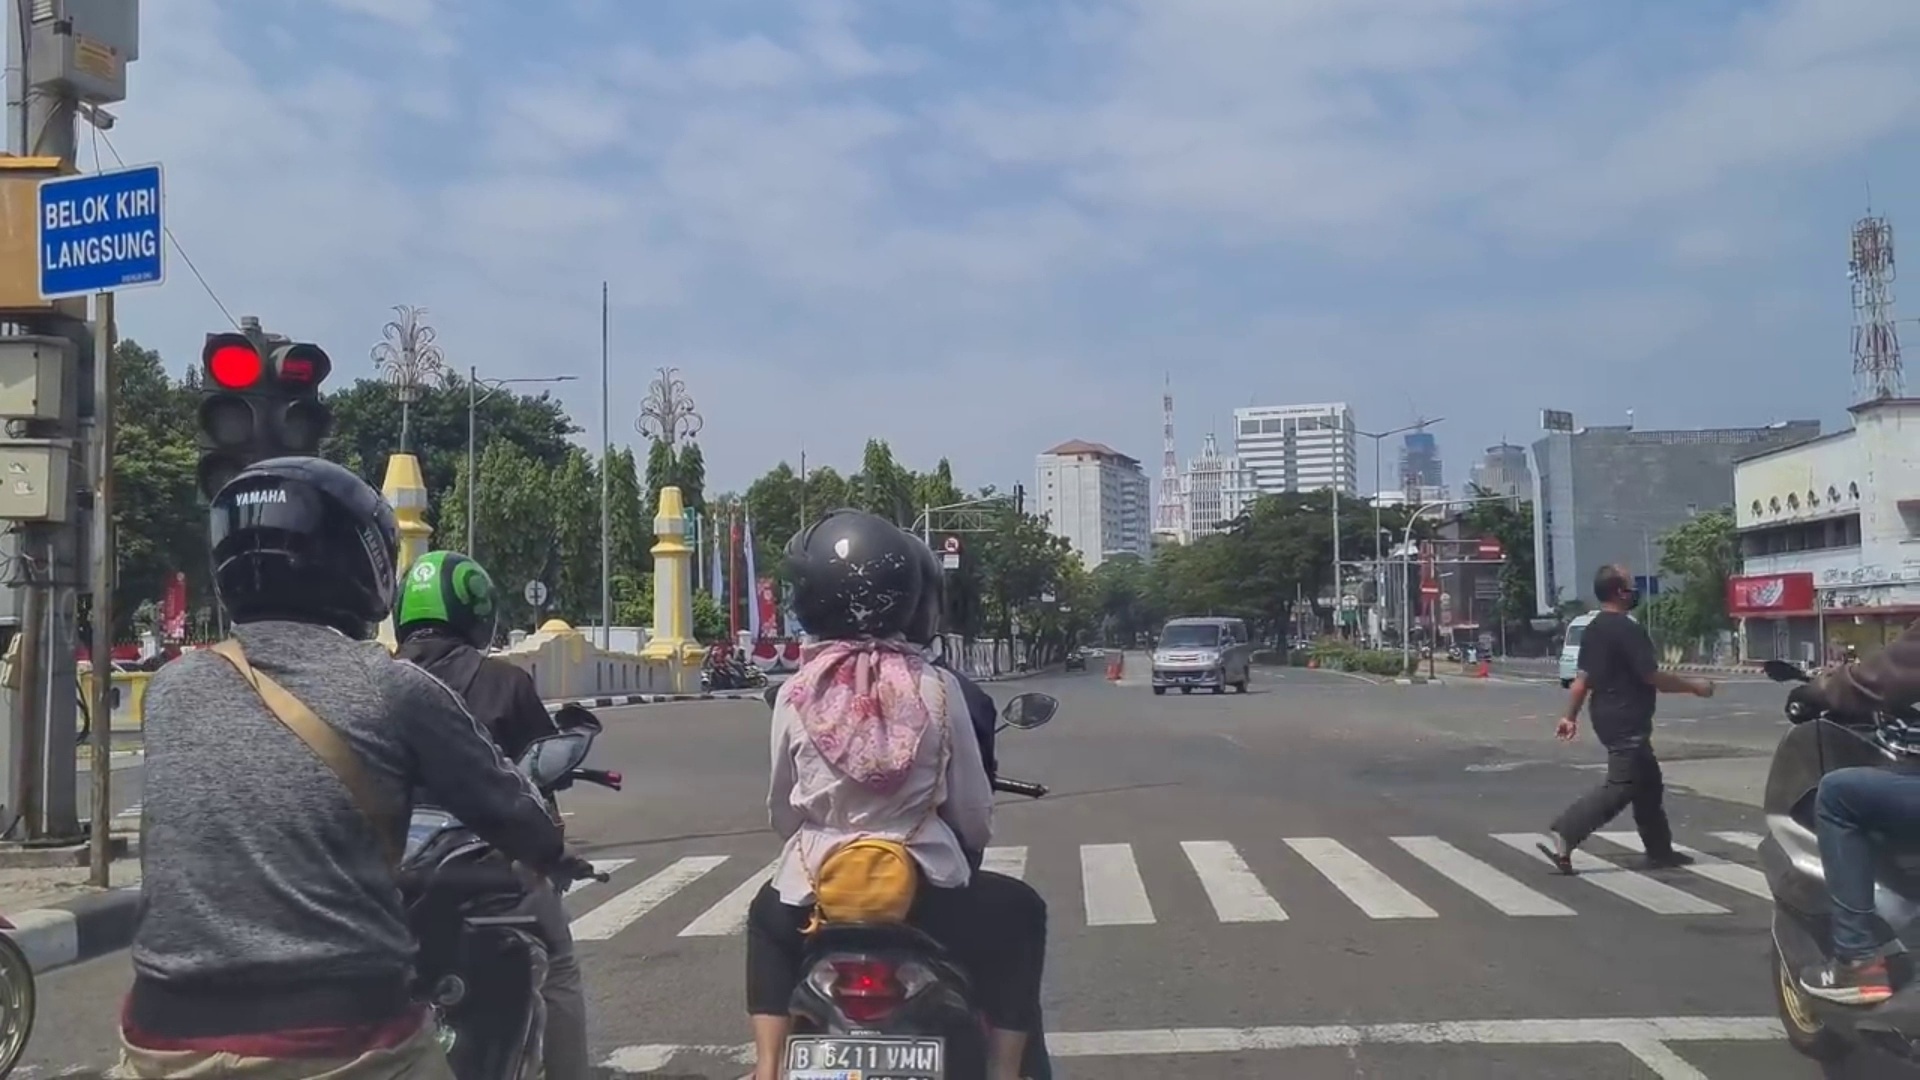
\includegraphics[width=\textwidth]{img/frame475.jpg}
			\caption*{(b) Siang}
		\end{minipage}
		\hfill
		\begin{minipage}[b]{0.2\textwidth}
			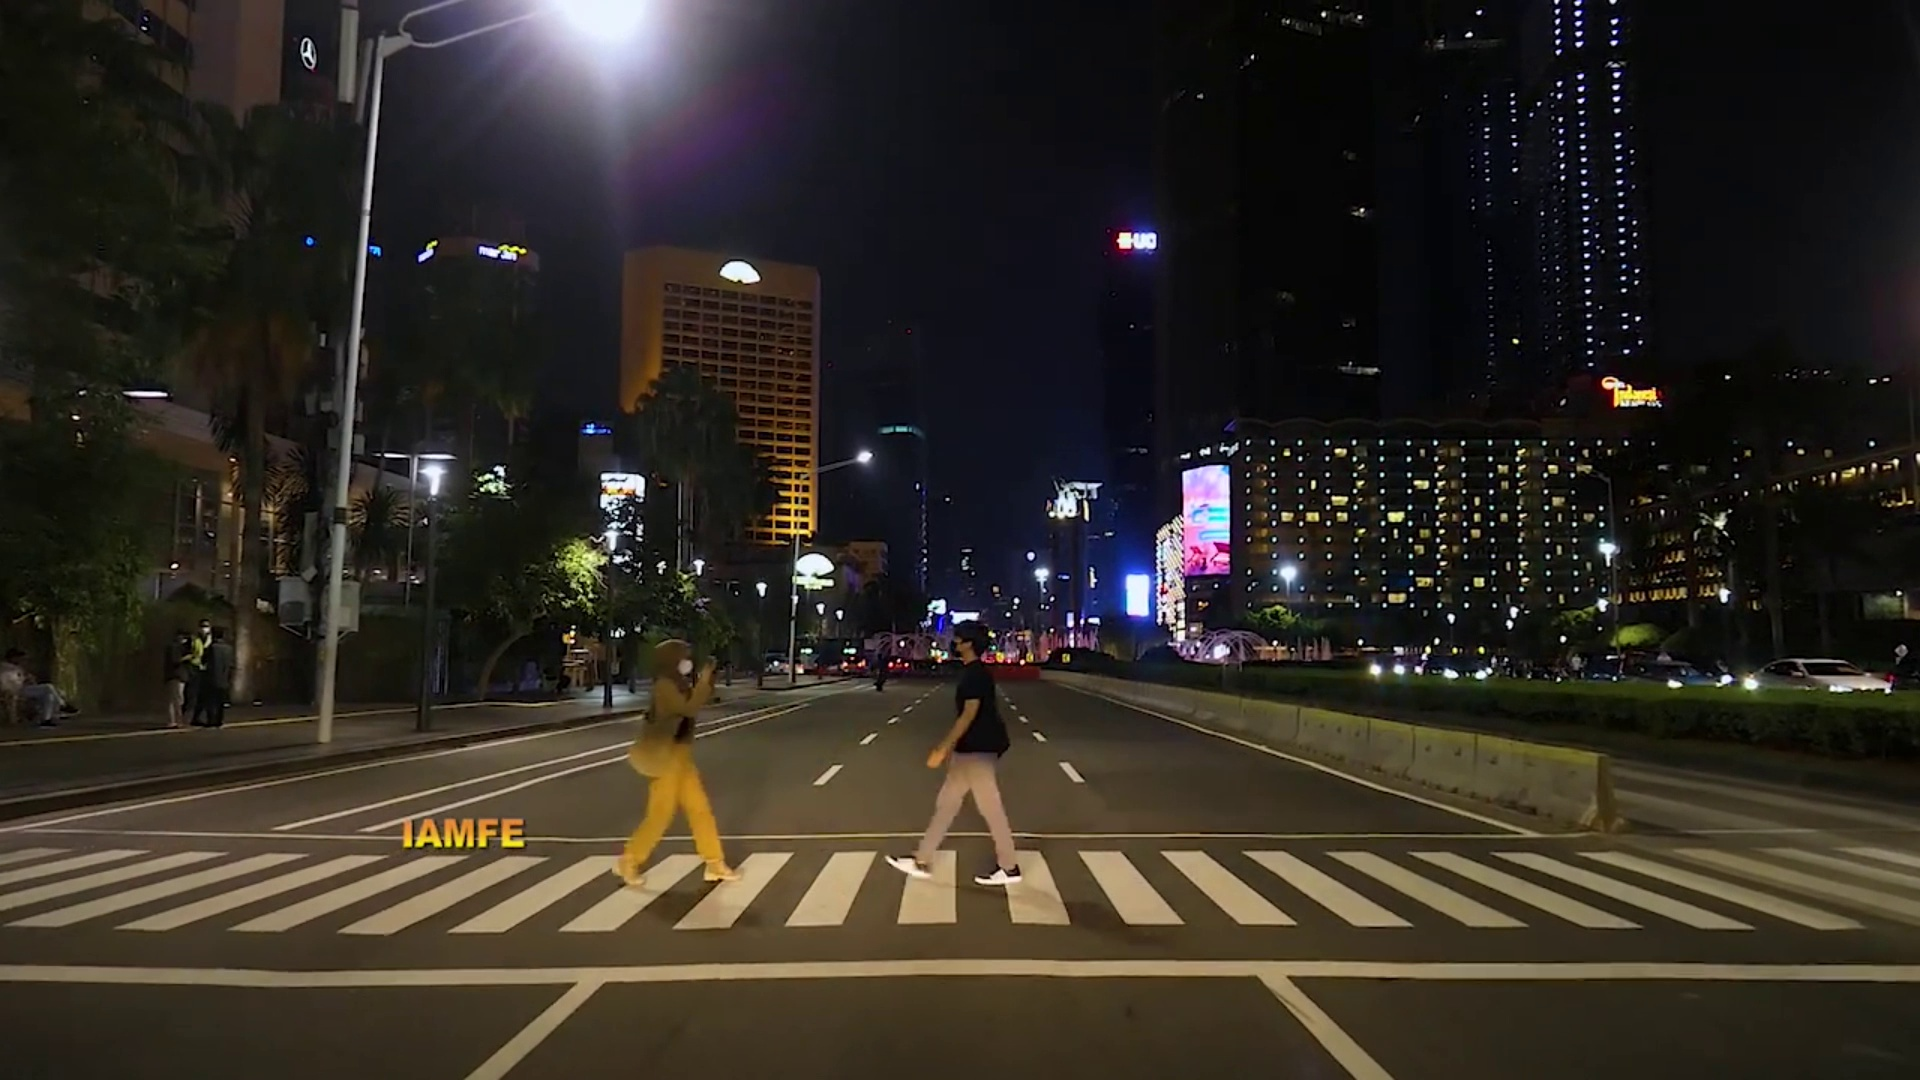
\includegraphics[width=\textwidth]{img/frame180.jpg}
			\caption*{(c) Malam}
		\end{minipage}
		\caption{{Gambar \textit{Testing} pada Kondisi yang Berbeda}}
		\label{fig:compare}
	\end{figure}

	\vspace{1ex}
	\begin{table}[h]
		\centering
		\begin{tabular}{|l|c|c|c|}
			\hline
			\multicolumn{1}{|c|}{\textit{\textbf{Backbone}}} & \textit{\textbf{mAP (\%)}} & \textit{\textbf{mAR (\%)}} & \textit{\textbf{F1 Score (\%)}} \\ \hline
			ResNet-50                                        & 66.785                     & 77                         & 71.529                          \\ \hline
			\textit{ResNet-101}                              & 76.605                     & 85.375                     & 90.302                          \\ \hline
			\textit{MobileNet-v1}                            & 25                         & Nan                        & Nan                             \\ \hline
		\end{tabular}
		\caption{Perbandingan Evaluasi Setiap Model}
		\label{tab:result}
	\end{table}
	
	\section{Conclusion}
	\vspace{1ex}
	Berdasarkan hasil pengujian yang telah dilakukan, penulis dapat menyimpulkan bahwa dalam penelitian ini telah diimplementasikan dengan baik proses deteksi dan segementasi pejalan kaki dan zebracross dengan menggunakan Mask R-CNN, dengan \textit{mean Average Precision} sebesar 76.62\%. {Backbone} ResNet-101 memiliki hasil akurasi yang lebih baik dibanding dengan \textit{backbone} lainnya dengan peforma lebih tinggi sebesar 12.82\% dibanding ResNet-50 dan 67.36\% dibanding MobileNet-v1. Waktu yang dibutuhkan dalam proses pendektesian akan semakin lama jika objek yang berada pada gambar semakin banyak. 
	
	\bibliographystyle{IEEEtran}
	\bibliography{dpustaka}
\end{document}
